\documentclass[aspectratio=169]{beamer}
\usetheme{Madrid}
\usecolortheme{default}

% Packages
\usepackage{tikz}
\usepackage{algorithm}
\usepackage{algorithmic}
\usepackage{amsmath}
\usepackage{amssymb}
\usepackage{booktabs}
\usepackage{graphicx}

% TikZ libraries
\usetikzlibrary{shapes,arrows,positioning,calc,backgrounds,fit,decorations.pathreplacing}

% Custom colors
\definecolor{maincolor}{RGB}{0,102,204}
\definecolor{accentcolor}{RGB}{255,102,0}
\definecolor{lightgray}{RGB}{240,240,240}
\definecolor{successcolor}{RGB}{46,125,50}

% Title information
\title[MOEA/D]{MOEA/D: A Multiobjective Evolutionary Algorithm\\Based on Decomposition}
\subtitle{An Intuitive Guide from Basics to Implementation}
\author{Based on Zhang \& Li (2007)}
\date{\today}

\begin{document}

% =============================================================================
% TITLE AND INTRODUCTION
% =============================================================================
% \begin{frame}
% \titlepage
% \end{frame}

% =============================================================================
% SECTION 4: HOW MOEA/D WORKS
% =============================================================================



% \section{ Speaker 3 — MOEA/D Architecture & Insight.}
% \begin{frame}{}
%      Speaker 3 — MOEA/D Architecture & Insight.
% \end{frame}
\subsection{ How MOEA/D Works}
\begin{frame}{MOEA/D Philosophy}
\begin{center}
\Large
\textbf{Two Key Ideas:}
\end{center}

\vspace{1em}
\pause
\begin{enumerate}
\item \textbf{Decomposition:} Break into simple problems
\begin{center}
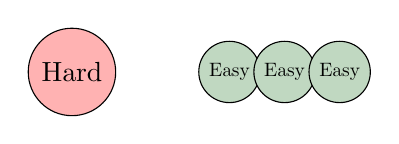
\begin{tikzpicture}
\node[draw,circle,fill=red!30] at (0,0) {Hard};
\foreach \x in {2,2.7,3.4} {
    \node[draw,circle,fill=successcolor!30,scale=0.7] at (\x,0) {Easy};
}
\end{tikzpicture}
\end{center}

\vspace{1em}
\pause
\item \textbf{Collaboration:} Let similar problems help each other
\begin{center}
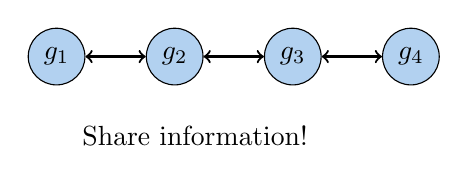
\begin{tikzpicture}
\foreach \i/\x in {1/0, 2/1.5, 3/3, 4/4.5} {
    \node[draw,circle,fill=maincolor!30] (n\i) at (\x,0) {$g_\i$};
}
\draw[<->,thick] (n1) -- (n2);
\draw[<->,thick] (n2) -- (n3);
\draw[<->,thick] (n3) -- (n4);
\node[below=0.5cm of n2.south east] {Share information!};
\end{tikzpicture}
\end{center}
\end{enumerate}
\end{frame}
%================================================================

\begin{frame}{Understanding MOEA/D: The 5 Friends Story}
\vspace{-2em}
\begin{center} \textbf{�� The 5 Friends - Each with Different Car Preferences} \end{center}
\pause
\begin{columns}[T]

%% ─── LEFT COLUMN ───────────────────────────────────────────
\begin{column}{0.50\textwidth}

  \vspace{0.4em}

  % ── Friends: one per line, vertical list ──────────────────
  {\small
  \textcolor{red!70!black}{\textbf{Friend 1}} \quad Quality first  (90\% Quality-10\% Price)

  \vspace{0.4em}
  \textcolor{orange!80!black}{\textbf{Friend 2}} \quad Good quality (70\% Quality-30\% Price)

  \vspace{0.4em}
  \textcolor{yellow!60!black}{\textbf{Friend 3}} \quad Balanced (50\% Quality-50\% Price)

  \vspace{0.4em}
  \textcolor{green!60!black}{\textbf{Friend 4}} \quad Cheaper car (30\% Quality-70\% Price)

  \vspace{0.4em}
  \textcolor{blue!80!black}{\textbf{Friend 5}} \quad Cheapest! (10\% Quality-90\% Price)
  }


  \vspace{1em}
  \pause

\begin{center}
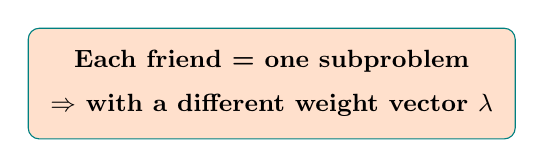
\begin{tikzpicture}
  \node[
    fill=accentcolor!20,
    draw=teal,
    rounded corners,
    inner sep=8pt,
    align=center
  ] {
    \textbf{\small Each friend = one subproblem}\\[0.4em]
    \textbf{\small $\Rightarrow$ with a different weight vector $\lambda$}
  };
\end{tikzpicture}
\end{center}

\end{column}

%% ─── RIGHT COLUMN ───────────────────────────────────────────
\begin{column}{0.48\textwidth}

  % ── Graph appears on Pause 3 ──────────────────────────────
  % \pause
  
  {\underline {INITIALIZATION:}}
  \vspace{-1em}
  \begin{center}
  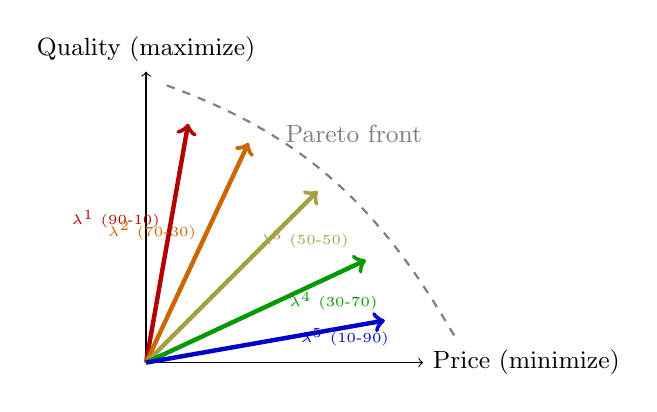
\begin{tikzpicture}[scale=0.88]
    \draw[->] (0,0) -- (4,0) node[right,font=\small] {Price (minimize)};
    \draw[->] (0,0) -- (0,4.2) node[above,font=\small] {Quality (maximize)};

    \draw[->,ultra thick,red!70!black]    (0,0) -- (80:3.5) node[pos=0.6,left,font=\tiny]       {$\lambda^1$ (90-10)};
    \draw[->,ultra thick,orange!80!black] (0,0) -- (65:3.5) node[pos=0.6,left,font=\tiny]       {$\lambda^2$ (70-30)};
    \draw[->,ultra thick,yellow!60!black] (0,0) -- (45:3.5) node[pos=0.6,above right,font=\tiny]{$\lambda^3$ (50-50)};
    \draw[->,ultra thick,green!60!black]  (0,0) -- (25:3.5) node[pos=0.6,right,font=\tiny]      {$\lambda^4$ (30-70)};
    \draw[->,ultra thick,blue!80!black]   (0,0) -- (10:3.5) node[pos=0.6,right,font=\tiny]      {$\lambda^5$ (10-90)};

    \draw[thick,gray,dashed] (0.3,4.0) to[out=-20,in=120] (4.5,0.3);
    \node[gray,font=\small] at (3.0,3.3) {Pareto front};
  \end{tikzpicture}
  \end{center}

\end{column}
\end{columns}

\end{frame}

%%%%%%%%%%%%%%%%%%%%%%%%%%%%%%%%%%%%%%%%%%%%%%%%%%%%%%%


\begin{frame}{Step 1: Random Initial Solution}

Each friend randomly picks one car from the \textbf{design space}\\

\vspace{0.5em}

\begin{center}
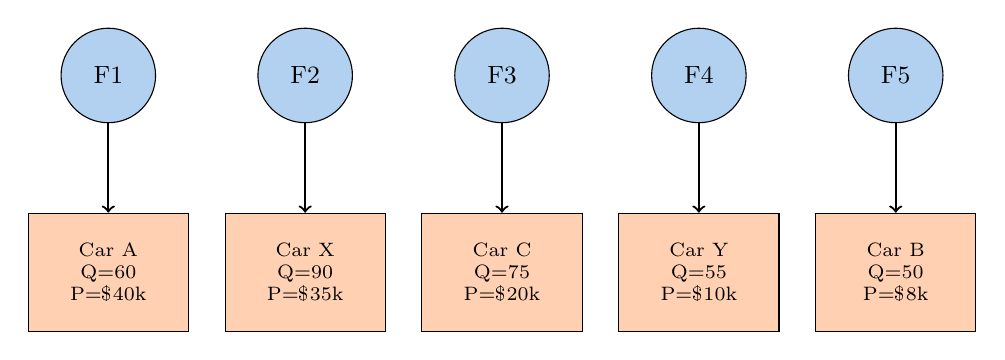
\begin{tikzpicture}[
    friend/.style={draw,circle,fill=maincolor!30,minimum size=1.2cm,font=\small},
    car/.style={draw,rectangle,fill=accentcolor!30,text width=1.8cm,minimum height=1.5cm,align=center,font=\scriptsize}
]
% Friend nodes
\node[friend] (g1) at (0,3) {F1};
\node[friend] (g2) at (2.5,3) {F2};
\node[friend] (g3) at (5,3) {F3};
\node[friend] (g4) at (7.5,3) {F4};
\node[friend] (g5) at (10,3) {F5};

\onslide<2->{
% Car nodes (solutions)
\node[car] (x1) at (0,0.5) {Car A\\Q=60\\P=\$40k};
\node[car] (x2) at (2.5,0.5) {Car X\\Q=90\\P=\$35k};
\node[car] (x3) at (5,0.5) {Car C\\Q=75\\P=\$20k};
\node[car] (x4) at (7.5,0.5) {Car Y\\Q=55\\P=\$10k};
\node[car] (x5) at (10,0.5) {Car B\\Q=50\\P=\$8k};

% Connections
\draw[->,thick] (g1) -- (x1);
\draw[->,thick] (g2) -- (x2);
\draw[->,thick] (g3) -- (x3);
\draw[->,thick] (g4) -- (x4);
\draw[->,thick] (g5) -- (x5);
}
\end{tikzpicture}
\end{center}

\vspace{0.5em}
\onslide<2->{
\begin{center}

\begin{tikzpicture}
\node[draw,rounded corners,fill=yellow!30,text width=9cm,align=center] {
% Each friend randomly picks one car from the design space\\
This creates the \textbf{initial population} of solutions
};
\end{tikzpicture}
\end{center}

}

\end{frame}



% \begin{frame}{STEP 3: Improve By Learning From Neighbors}

% \begin{center}
% \textbf{Friend 3 wants a better car — so he studies his neighbors!}
% \end{center}

% \vspace{0.4em}

% \begin{columns}[T]

% %% ─── LEFT COLUMN: the situation ────────────────────────────
% \begin{column}{0.48\textwidth}

%   \begin{tikzpicture}[
%       friend/.style={draw,circle,fill=maincolor!30,minimum size=1.1cm,font=\small},
%       car/.style={draw,rectangle,rounded corners,text width=2cm,
%                   minimum height=1.4cm,align=center,font=\scriptsize}
%   ]
%     % Three friends only
%     \node[friend,fill=orange!30]      (g2) at (0,3)   {F2};
%     \node[friend,fill=maincolor!50]   (g3) at (3,3)   {F3};
%     \node[friend,fill=green!30]       (g4) at (6,3)   {F4};

%     % Their cars
%     \node[car,fill=orange!20]  (x2) at (0,0.8)
%         {\textbf{Car X}\\Q=90\\P=\$35k\\{\tiny High Q, Costly}};
%     \node[car,fill=maincolor!20] (x3) at (3,0.8)
%         {\textbf{Car C}\\Q=75\\P=\$20k\\{\tiny Current}};
%     \node[car,fill=green!20]   (x4) at (6,0.8)
%         {\textbf{Car Y}\\Q=55\\P=\$10k\\{\tiny Cheap, Med Q}};

%     % Friend → Car
%     \draw[->,thick] (g2) -- (x2);
%     \draw[->,thick] (g3) -- (x3);
%     \draw[->,thick] (g4) -- (x4);

%     % F3 looks at neighbors
%     \onslide<2->{\draw[->,thick,red,dashed] (x2) to[bend right=25] (g3);}
%     \onslide<3->{\draw[->,thick,red,dashed] (x4) to[bend left=25]  (g3);}

%     % Thought bubble label
%     \onslide<4->{\node[draw,rounded corners,fill=yellow!20,font=\scriptsize,
%           text width=3cm,align=center] at (3,-0.9)
%         {\textit{``What if I find\\something in between?''}};
%     \draw[->,gray,dashed] (g3.south) -- (3,-0.5);}

%   \end{tikzpicture}

% \end{column}

% %% ─── RIGHT COLUMN: the result ──────────────────────────────
% \begin{column}{0.48\textwidth}
%   \begin{center}
%   \vspace{0.5em}

%   % Step-by-step reasoning
%   {\small
%   \onslide<2->{\textcolor{orange!80!black}{\textbf{F2's car:}} High quality, but expensive\\[4pt]}
%   \onslide<3->{\textcolor{green!60!black}{\textbf{F4's car:}} Cheap, but medium quality\\[4pt]}
%  \onslide<4->{ \textcolor{maincolor}{\textbf{F3 thinks:}} \textit{``Find something in between!''}}
%   }

%   \vspace{0.8em}
   
%   \end{center}
% \end{column}
% \end{columns}

% \end{frame}







\begin{frame}{STEP 2: Crossover+Mutation — Combining Ideas From Neighbors}

\begin{center}
\textbf{Friend 3 takes parts from both neighbors' cars to build a new one}
\end{center}

\begin{center}
\resizebox{\textwidth}{!}{
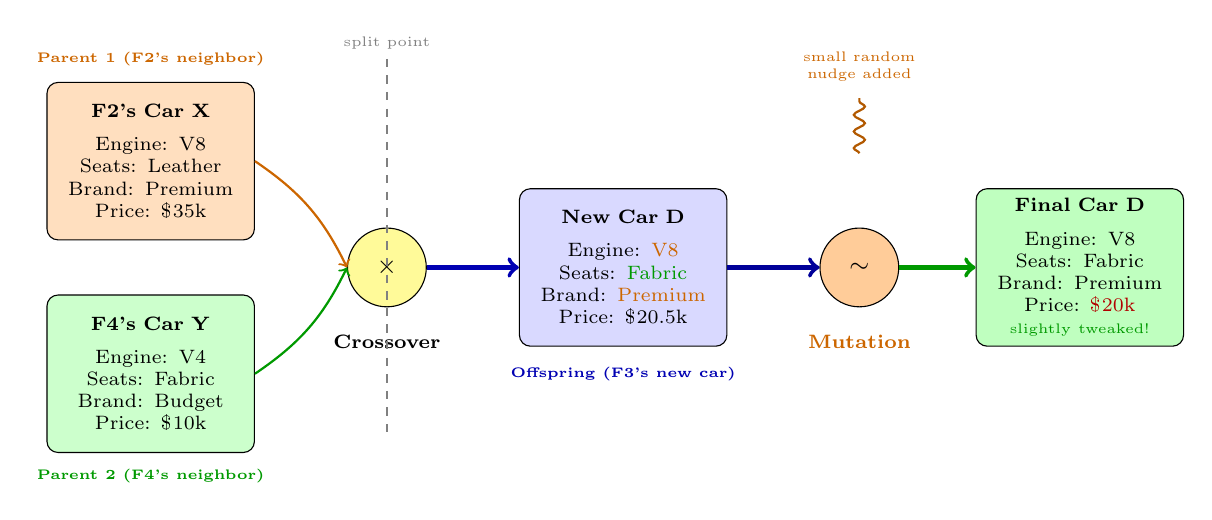
\begin{tikzpicture}[
    car/.style={draw,rectangle,rounded corners,text width=2.4cm,
                minimum height=2.0cm,align=center,font=\scriptsize},
    gene/.style={draw,rectangle,minimum width=2.4cm,minimum height=0.55cm,
                 align=center,font=\scriptsize}
]

  % Parent 1 — F2's car
  \node[car,fill=orange!25] (p1) at (0,3.2) {
    \textbf{F2's Car X}\\[4pt]
    Engine: V8\\
    Seats: Leather\\
    Brand: Premium\\
    Price: \$35k
  };

  % Parent 2 — F4's car
  \node[car,fill=green!20] (p2) at (0,0.5) {
    \textbf{F4's Car Y}\\[4pt]
    Engine: V4\\
    Seats: Fabric\\
    Brand: Budget\\
    Price: \$10k
  };

\onslide<2->{
  % Crossover operator
  \node[draw,circle,fill=yellow!40,minimum size=1.0cm,
        font=\small\bfseries] (cross) at (3.0,1.85) {$\times$};

  \draw[->,thick,orange!80!black] (p1.east) to[bend left=15]  (cross.west);
  \draw[->,thick,green!60!black]  (p2.east) to[bend right=15] (cross.west);
}

\onslide<2->{
  % Child car
  \node[car,fill=blue!15] (child) at (6.0,1.85) {
    \textbf{New Car D}\\[4pt]
    Engine: \textcolor{orange!80!black}{V8}\\
    Seats: \textcolor{green!60!black}{Fabric}\\
    Brand: \textcolor{orange!80!black}{Premium}\\
    Price: \$20.5k
  };

  \draw[->,ultra thick,blue!70!black] (cross.east) -- (child.west);
}

  % Labels
  \node[font=\tiny,orange!80!black] at (0, 4.5)  {\textbf{Parent 1 (F2's neighbor)}};
  \node[font=\tiny,green!60!black]  at (0, -0.8) {\textbf{Parent 2 (F4's neighbor)}};
  \onslide<3->{\node[font=\tiny,blue!70!black] at (6.0,0.5){\textbf{Offspring (F3's new car)}};}

\onslide<2->{
  \node[font=\scriptsize\bfseries] at (3.0, 0.9) {Crossover};

  % Crossover point line
  \draw[thick,dashed,gray] (3.0,4.5) -- (3.0,-0.3);
  \node[font=\tiny,gray] at (3.0,4.7) {split point};
}

\onslide<3->{
  % Mutation operator — on the same horizontal line as child (y=1.85)
  \node[draw,circle,fill=orange!40,minimum size=1.0cm,
        font=\small\bfseries] (mut) at (9.0,1.85) {$\sim$};

  \draw[->,ultra thick,blue!60!black] (child.east) -- (mut.west);
}

\onslide<3->{
  % After mutation — same horizontal line (y=1.85)
  \node[car,fill=green!25] (after) at (11.8,1.85) {
    \textbf{Final Car D}\\[4pt]
    Engine: V8\\
    Seats: Fabric\\
    Brand: Premium\\
    Price: \textcolor{red!70!black}{\$20k}\\
    \textcolor{green!60!black}{\tiny slightly tweaked!}
  };

  \draw[->,ultra thick,green!60!black] (mut.east) -- (after.west);
}

\onslide<3->{  % Mutation label
  \node[font=\scriptsize\bfseries,orange!80!black] at (9,0.9) {Mutation};

% Mutation = small random nudge
  \draw[decorate,decoration={snake,amplitude=2pt,segment length=6pt},
        thick,orange!70!black]
       (9,3.3) -- (9,4.0);
  \node[font=\tiny,orange!80!black,align=center] at (9,4.4)
       {small random\\nudge added};}

\end{tikzpicture}
}
\end{center}

\end{frame}

%%%%%%%%%%%%%%%%%%%%%%%%%%%%%%%%%%%%%%%%%%%

\begin{frame}{Step 3: Does Car D Actually Help the Neighbors?}

\begin{center}
\textbf{Friend 3 shares Car D — each neighbor checks if it beats their current car}
\end{center}

\vspace{0.2em}

\begin{center}
\begin{tikzpicture}[scale=0.9]

  % ── Pause 1: Car D star ───────────────────────────────────
\node[draw,rectangle,fill=green!50,minimum width=2.0cm,
        minimum height=1.0cm,align=center,font=\scriptsize]
        (y) at (0,4.5) {Car D\\Q=80, \$20k};


  
  % ── Pause 2: friends + cars (old) + weight labels ─────────
  % \pause
    \onslide<2->{
  \node[font=\tiny,orange!80!black] at (-3,  2.85) {70\% Quality};
  \node[font=\tiny,maincolor]       at ( 0,  2.85) {50\%--50\%};
  \node[font=\tiny,green!60!black]  at ( 3,  2.85) {70\% Price};

  \node[draw,circle,fill=orange!30,minimum size=1.1cm,font=\small]
        (g2) at (-3,2) {F2};
  \node[draw,circle,fill=maincolor!50,minimum size=1.1cm,font=\small]
        (g3) at ( 0,2) {F3};
  \node[draw,circle,fill=orange!30,minimum size=1.1cm,font=\small]
        (g4) at ( 3,2) {F4};

  \node[draw,rectangle,fill=orange!15,minimum width=2.0cm,
        minimum height=1.0cm,align=center,font=\scriptsize]
        (x4) at ( 3,0) {Car Y\\Q=55, \$10k};
    }
    % \onslide<3-5>{
  % Old cars
\onslide<2-5>{  \node[draw,rectangle,fill=orange!15,minimum width=2.0cm,
        minimum height=1.0cm,align=center,font=\scriptsize]
        (x2) at (-3,0) {Car X\\Q=90, \$35k};}
\onslide<2-8>{  \node[draw,rectangle,fill=maincolor!20,minimum width=2.0cm,
        minimum height=1.0cm,align=center,font=\scriptsize]
        (x3) at ( 0,0) {Car C\\Q=75, \$20k};}
% }
    \onslide<2->{
  \draw[->,thick] (g2) -- (x2);
  \draw[->,thick] (g3) -- (x3);
  \draw[->,thick] (g4) -- (x4);
}
  % ── Pause 3: blue arrows + rule note ─────────────────────
  % \pause
  % \onslide<4->{

 \onslide<3-5>{ \draw[->,thick,blue] (y) to[out=-90,in=90] (g2);}
\onslide<6-8>{  \draw[->,thick,blue] (y) to[out=-90,in=90] (g3);}
\onslide<9-11>{  \draw[->,thick,blue] (y) to[out=-90,in=90] (g4);}

\only<3-5>{
  \begin{scope}[on background layer]
    \draw[draw=blue!70, line width=1pt, rounded corners=6pt,
          fill=blue!10, fill opacity=0.6]
          (-4.3,-0.7) rectangle (-1.7,3.1);
    \node[font=\tiny, blue!80] at (-3, 3.3) {Comparing...};
  \end{scope}
}

% ── Spotlight: Car D vs Car C ─────────────────
\only<6-8>{
  \begin{scope}[on background layer]
    \draw[draw=blue!70, line width=1pt, rounded corners=6pt,
          fill=blue!10, fill opacity=0.6]
          (-1.3,-0.7) rectangle (1.3,3.1);
    \node[font=\tiny, blue!80] at (0, 3.3) {Comparing...};
  \end{scope}
}
% ── Spotlight: Car D vs Car Y ─────────────────
\only<9-10>{
  \begin{scope}[on background layer]
    \draw[draw=blue!70, line width=1pt, rounded corners=6pt,
          fill=blue!10, fill opacity=0.6]
          (1.7,-0.7) rectangle (4.3,3.1);
    \node[font=\tiny, blue!80] at (3, 3.3) {Comparing...};
  \end{scope}
}



  
 \onslide<2->{
  \node[draw,rounded corners,fill=yellow!30,text width=2cm,
        align=center,font=\scriptsize] at (6.6,3.2)
        {Car D replaces only if it scores \textbf{better} by
         \textbf{that friend's own weights}};
  \draw[->,gray,dashed] (5.25,3.2) -- (1.2,3.2);
}
  % ── Pause 4: replace/keep arrows ─────────────────────────
  % \pause
  % \onslide<5->{

\onslide<4>{  \draw[->,ultra thick,green!60!black] (x2) -- ++(0,-0.9)
        node[below,font=\scriptsize,green!60!black] {\textbf{Replace! ✓}};}
\onslide<7>{  \draw[->,ultra thick,green!60!black] (x3) -- ++(0,-0.9)
        node[below,font=\scriptsize,green!60!black] {\textbf{Replace! ✓}};}
\onslide<10>{  \draw[->,ultra thick,red!70!black]   (x4) -- ++(0,-0.9)
        node[below,font=\scriptsize,red!70!black]   {\textbf{Keep old ✗}};}
% }
  % ── Pause 5: updated cars (Car D replaces X and C) ────────
  % \pause
    % \onslide<6->{
\onslide<5->{  \node[draw,rectangle,fill=green!50,minimum width=2.0cm,
        minimum height=1.0cm,align=center,font=\scriptsize]
        at (-3,0) {Car D\\Q=80, \$20k};}
\onslide<8->{  \node[draw,rectangle,fill=green!50,minimum width=2.0cm,
        minimum height=1.0cm,align=center,font=\scriptsize]
        at ( 0,0) {Car D\\Q=80, \$20k};}
% }
  % ── Pause 6: takeaway ────────────────────────────────────
  % \pause
  \onslide<11->{

  \node[draw,rounded corners,fill=green!30,text width=2cm,
        align=center,font=\scriptsize] at (6.6,0)
        {So one \textbf{good discovery} can help multiple nearby subproblems.};
}

\end{tikzpicture}
\end{center}

\end{frame}



%%%%%%%%%%%%%%%%%%%%%%%%%%%%%%%%%%%%%%%%%%%%%%%%%%%%%%%%%%%%%%%%5
\begin{frame}{Step 4: Repeat Many Times — Everyone Keeps Improving}

\begin{center}
\textbf{Each friend takes turns — look at neighbors, try new car, replace if better}
\end{center}

\vspace{0.2em}

\begin{center}
\begin{tikzpicture}[scale=1]

  % ── All 5 friends + their cars (shown from start) ─────────
  \node[draw,circle,fill=red!25,minimum size=1.1cm,font=\small]
        (g1) at (-4,2) {F1};
  \node[draw,circle,fill=orange!30,minimum size=1.1cm,font=\small]
        (g2) at (-2,2) {F2};
  \node[draw,circle,fill=maincolor!50,minimum size=1.1cm,font=\small]
        (g3) at ( 0,2) {F3};
  \node[draw,circle,fill=green!30,minimum size=1.1cm,font=\small]
        (g4) at ( 2,2) {F4};
  \node[draw,circle,fill=blue!25,minimum size=1.1cm,font=\small]
        (g5) at ( 4,2) {F5};

  % Weight labels
  \node[font=\tiny,red!70!black]    at (-4,3.1) {90\% Quality};
  \node[font=\tiny,orange!80!black] at (-2,3.1) {70\% Quality};
  \node[font=\tiny,maincolor]       at ( 0,3.1) {50\%--50\%};
  \node[font=\tiny,green!60!black]  at ( 2,3.1) {70\% Price};
  \node[font=\tiny,blue!70!black]   at ( 4,3.1) {90\% Price};

  % Current best cars
  \node[draw,rectangle,fill=red!15,minimum width=1.8cm,
        minimum height=0.9cm,align=center,font=\scriptsize]
        (x1) at (-4,0) {Car A\\Q=60};
  \node[draw,rectangle,fill=orange!15,minimum width=1.8cm,
        minimum height=0.9cm,align=center,font=\scriptsize]
        (x2) at (-2,0) {Car D\\Q=80};
  \node[draw,rectangle,fill=maincolor!20,minimum width=1.8cm,
        minimum height=0.9cm,align=center,font=\scriptsize]
        (x3) at ( 0,0) {Car D\\Q=80};
  \node[draw,rectangle,fill=green!15,minimum width=1.8cm,
        minimum height=0.9cm,align=center,font=\scriptsize]
        (x4) at ( 2,0) {Car Y\\Q=55};
  \node[draw,rectangle,fill=blue!15,minimum width=1.8cm,
        minimum height=0.9cm,align=center,font=\scriptsize]
        (x5) at ( 4,0) {Car B\\Q=50};

  \draw[->,thick] (g1)--(x1);
  \draw[->,thick] (g2)--(x2);
  \draw[->,thick] (g3)--(x3);
  \draw[->,thick] (g4)--(x4);
  \draw[->,thick] (g5)--(x5);

  % ── Pause 1: F4 takes turn ────────────────────────────────
  \onslide<2->{
  \node[draw,dashed,rounded corners,green!60!black,
        minimum width=1.4cm,minimum height=1.4cm] at (2,2) {};
  \node[font=\tiny,green!60!black] at (2,1.1) {\textbf{My turn!}};

  \draw[->,thick,green!60!black,dashed] (g3) to[bend left=20]  (g4);
  \draw[->,thick,green!60!black,dashed] (g5) to[bend right=20] (g4);
  }

  % ── Pause 2: F4 updates ───────────────────────────────────
  \onslide<3->{
  \node[draw,rectangle,fill=green!30,minimum width=1.8cm,
        minimum height=0.9cm,align=center,font=\scriptsize]
        at (2,0) {\textbf{Car E}\\\$12k};
  \draw[->,ultra thick,green!60!black] (g4) -- (x4))
        node[right,font=\tiny,green!60!black,pos=0.5] {improved!};
  }

  % ── Pause 3: F1 takes turn ────────────────────────────────
  \onslide<4->{
  \node[draw,dashed,rounded corners,red!70!black,
        minimum width=1.4cm,minimum height=1.4cm] at (-4,2) {};
  \node[font=\tiny,red!70!black] at (-4,1.1) {\textbf{My turn!}};

  \draw[->,thick,red!60,dashed] (g2) to[bend right=20] (g1);
  }

  % ── Pause 4: F5 takes turn ────────────────────────────────
  \onslide<5->{
  \node[draw,dashed,rounded corners,blue!70!black,
        minimum width=1.4cm,minimum height=1.4cm] at (4,2) {};
  \node[font=\tiny,blue!70!black] at (4,1.1) {\textbf{My turn!}};

  \draw[->,thick,blue!60,dashed] (g4) to[bend left=20] (g5);
  }

  % ── Pause 5: final result ─────────────────────────────────
  \onslide<6->{
  % Converged cars for all
  \node[draw,rectangle,fill=red!30,minimum width=1.8cm,
        minimum height=0.9cm,align=center,font=\scriptsize]
        at (-4,0) {\textbf{Best A+}\\Q=97};
  \node[draw,rectangle,fill=blue!25,minimum width=1.8cm,
        minimum height=0.9cm,align=center,font=\scriptsize]
        at ( 4,0) {\textbf{Best B+}\\\$7k};

  % Converged label above
  \node[draw,rounded corners,fill=yellow!30,text width=8.5cm,
        align=center,font=\scriptsize] at (0,4.4)
        {After many rounds $\rightarrow$ each friend has the \textbf{best possible car}
         for \textit{their own preference} $=$ one point on the \textbf{Pareto front}};
  }
\end{tikzpicture}
\end{center}

\end{frame}

%%%%%%%%%%%%%%%%%%%%%%%%%%%%%%%%%%%%%%%%%%%%%%%%%%%%%%







\begin{frame}{Why is MOEA/D \textit{Evolutionary}? — The Main Loop}
\begin{center}
\scalebox{0.75}{
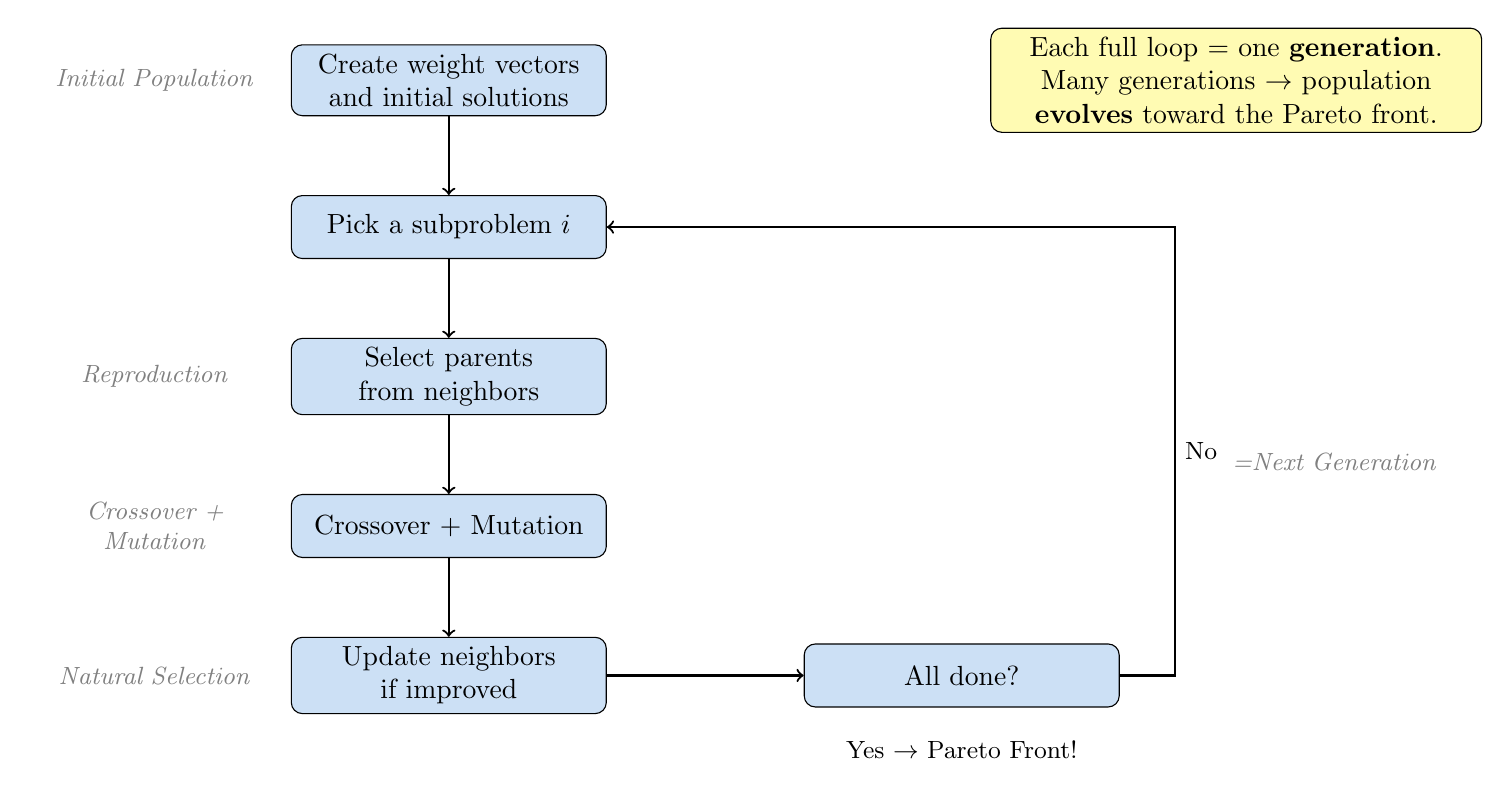
\begin{tikzpicture}[
    box/.style={rectangle, rounded corners, draw, fill=maincolor!20,
                minimum width=4cm, minimum height=0.8cm, align=center},
    evo/.style={font=\small, gray, text width=3cm, align=center},
    node distance=1cm
]

% ── Main loop boxes ───────────────────────────────────────
\node[box] (start)    {Create weight vectors\\and initial solutions};
\node[box, below=of start]    (select)   {Pick a subproblem $i$};
\node[box, below=of select]   (parents)  {Select parents\\from neighbors};
\node[box, below=of parents]  (offspring){Crossover + Mutation};
\node[box, below=of offspring](update)   {Update neighbors\\if improved};
\node[box, right=2.5cm of update] (check){All done?};

\onslide<2->{% ── Yellow box top-right ──────────────────────────────────
\node[draw, rounded corners, fill=yellow!30, font=\normalsize,
      text width=6cm, align=center] at (10, 0)
      {Each full loop = one \textbf{generation}.\\
       Many generations $\rightarrow$ population \textbf{evolves} toward the Pareto front.}
       ;}

\onslide<2->{% ── Evolutionary labels ─────────────────────
\node[evo, left=0.1cm of start]    {\textit{Initial Population}};
\node[evo, left=0.1cm of parents]  {\textit{Reproduction}};
\node[evo, left=0.1cm of offspring]{\textit{Crossover + Mutation}};
\node[evo, left=0.1cm of update]{\textit{Natural Selection}};
\node[evo] at (11.2, -4.843) {\textit{ =Next Generation}};
}
% ── Arrows ────────────────────────────────────────────────
\draw[->,thick] (start)    -- (select);
\draw[->,thick] (select)   -- (parents);
\draw[->,thick] (parents)  -- (offspring);
\draw[->,thick] (offspring)-- (update);
\draw[->,thick] (update)   -- (check);
\draw[->,thick] (check.east) -- ++(0.7,0) 
      |- node[near start, right, font=\small] {No} (select.east);

\node[below=0.3cm of check, font=\small] {Yes $\rightarrow$ Pareto Front!};

\end{tikzpicture}
}
\end{center}
\end{frame}

\begin{frame}{Conclusion}
    \vspace{1cm}
    \begin{center}
        \Large \textcolor{maincolor}{\textit{``Nothing is particularly hard if you divide it into small jobs.''}} \\[0.5cm]
        \normalsize -- Henry Ford \\[1.5cm]
        
        \Huge \textbf{Thank You!} \\[0.5cm]
        % \large Any Questions?
    \end{center}
\end{frame}


\end{document}
